\documentclass[letterpaper]{article}
\usepackage[spanish]{babel}
\selectlanguage{spanish}
\usepackage[utf8]{inputenc}

\usepackage{lipsum}
\usepackage{amsmath,amssymb,amsfonts,amsbsy}
\usepackage{array}
\usepackage{graphicx}
\usepackage{subfigure}
\usepackage{float}
%\usepackage{hyperref}
\usepackage[document]{ragged2e}
\usepackage{amsmath}
\usepackage{graphicx}
\graphicspath{ {./figures/} }

%\usepackage[pass]{geometry}
\usepackage[left=1.25in,right=1.25in,top=1.0in,bottom=1.0in]{geometry}
\usepackage{listings}
\usepackage{booktabs}
% Custom colors
\usepackage{color}
\definecolor{deepblue}{rgb}{0,0,0.65}
\definecolor{deepred}{rgb}{0.7,0,0}
\definecolor{deepgreen}{rgb}{0,0.6,0}

\usepackage{hyperref}
\hypersetup{
    colorlinks,
    citecolor=red,
    filecolor=red,
    linkcolor=black,
    urlcolor=black
}





\begin{document}

\nocite{*}

\begin{minipage}[t]{.13\textwidth}
	\vspace{-0.25in}
	\begin{figure}[H]
	
\includegraphics[width=0.90\textwidth]{LogoUC.jpg}
	\end{figure}
\end{minipage}
\hfill
\begin{minipage}[t]{.85\textwidth}
    \vspace{0pt}
    \begin{flushleft}
      \begin{tabular}{l}
	{\sc Pontificia Universidad Cat\'olica de Chile}\\
  	{\sc Escuela de Ingenier\'ia}\\
  	{\sc Departamento de Ingenier\'ia Industrial y Sistemas}\\
 	 {\sc ICS1113-Optimizaci\'on}
 \end{tabular}
	\end{flushleft}
\end{minipage}
\vspace{0pt}
\hfill
\vspace*{6cm}
\begin{center}{}
\vspace*{2mm}
{\Huge\bf Informe 3}\\
\vspace*{4mm}
\hrule\vspace*{1pt}\hrule
\vspace*{4mm}
{\LARGE\bf Desarrollo Inmobiliario Sustentable}\\
\vspace*{4mm}
{\huge\bf Grupo 65 }\\
\vspace*{1mm}
\end{center}

\vspace*{30mm}
\flushright 
	
Felipe Fuentes 	21637806  sección 3 \\
Victoria Hofmann 	21637385  sección 3\\
Vicente Pareja 	21637245 sección 2\\
Pedro Palma 	20639171  sección 1\\
Martín Campos 	21640874  sección 3\\
Francisco Solís  21638179  sección 2\\

 
\vspace*{5mm}
{\large Fecha entrega: 22 de Junio de 2022\\}
\flushleft
\newpage

\tableofcontents

\newpage

\section{Descripción del problema}


\subsection{Contexto}
\justify
Actualmente el cambio climático corresponde a uno de los desafíos más importantes a los que se enfrenta la humanidad. Si bien es un proceso natural,
la actividad antropogénica lo ha acelerado drásticamente, principalmente por la emisión de ciertos gases, llamados gases de efecto invernadero,
en donde uno de los principales es el dióxido de carbono\footnote{Causes of Climate Change, s.f.}. En caso de no reducir la huella de carbono de la actividad humana,
nos podemos ver enfrentados a consecuencias catastróficas en un futuro cercano. 
%Revisado el contexto - Francisco 18:43 23/05
\newline \newline
Es en este contexto, en donde el sector de la construcción toma protagonismo, al ser responsable de contribuir al 39\% de las emisiones de dióxido
de carbono relacionadas con la energía y procesos\footnote{Global Status Report for Buildings and Construction 2019 – Analysis. (s. f.). IEA.}. Por si ello fuese poco, esta
industria es responsable del 16\% del consumo mundial del agua\footnote{Enshassi, A., Kochendoerfer, B., \& Rizq, E. (2014). Evaluación de los impactos medioambientales de los proyectos de construcción. Revista ingeniería de construcción, 29(3), 234-254.}. Si bien la construcción es un sector que contamina en grandes cantidades, a su vez
aporta enormemente al desarrollo socioeconómico de un país, es más, es tal su importancia, que el 10\% de la economía mundial está dedicada a esta industria\footnote{Hill, R. C., \& Bowen, P. A. (1997). Sustainable construction: principles and a framework for attainment. Construction Management \& Economics, 15(3), 223-239.}.
Se espera que continúe su desarrollo, debido a que se estima que para poder ubicar a todas las personas que van a vivir en los sectores urbanos en el año 2060, se van a
tener que construir 230 mil millones de $m^{2}$ de nueva superficie\footnote{Why the building sector?, s. f.}. Lo anterior, deja en evidencia la necesidad de albergar
a una población que aumenta sostenidamente, pero sin descuidar los desafíos de sustentabilidad atingentes. \newline \newline
Además, a todo proyecto de construcción, se encuentra asociada la contaminación por polvo, operaciones que afectan la vegetación, contaminación atmosférica, contaminación
acústica y alta generación de residuos, entre otros.\newline \newline
Considerando estos factores, desafíos y objetivos climáticos, para llegar a la carbono neutralidad el año 2050, la Agencia Internacional de Energía (IEA) estima
que la emisión directa de dióxido de carbono producida por el sector de la construcción, tiene que reducirse a la mitad para el año 2030\footnote{Zhongming, Z., Linong, L., Xiaona, Y., Wangqiang, Z., \& Wei, L. (2020). Building sector emissions hit record high, but low-carbon pandemic recovery can help transform sector–UN report.}. Esto hace imperativo una tranformación de la industria de la construcción, para que así sea sostenible a lo largo del tiempo.
%Revisado hasta acá - Francisco 18:58 23/05
\subsection{Importancia de resolverlo}
El problema que este proyecto busca resolver es sumamente importante puesto que la construcción produce muchos residuos que afectan significativamente al medioambiente.
Además, hay diversos desafíos que se deben superar al intentar suplir la demanda habitacional sin perjudicar al medioambiente que nuestro proyecto busca superar, como el uso
de espacios y recursos, y la contaminación. Específicamente,  el proyecto se centra en la reducción de las emisiones de dióxido de carbono puesto que es de los gases de efecto
invernadero que más se emite en la industria de la construcción y es de los más influyentes en el cambio climático. Es así como se busca resolver un problema
que abarca diversas aristas, pues apunta a reducir la contaminación por emisiones al planificar un proyecto inmobiliario, al mismo tiempo que busca cumplir con ciertas
características. Otro rasgo importante a tener en consideración es que este proyecto puede tener un gran impacto en la búsqueda a nivel nacional y global por alcanzar la
carbono neutralidad, mediante la reducción de emisiones de dióxido de carbono en la construcción. Si bien es difícil indicar numéricamente el efecto que nuestro proyecto
puede generar en las emisiones, es posible estimarlo sabiendo el rol que juega la reducción de las emisiones debido a la construcción en la búsqueda de la carbono neutralidad.
Específicamente, se espera que en Chile se logre reducir en un 45\% las emisiones de dióxido de carbono (respecto al 2016) para el año 2030 con el objetivo de alcanzar
la carbono neutralidad en el año 2050. Si se considera que la industria de la construcción conforma el 23\% de las emisiones de $CO_{2}$ en Chile, es posible decir que
se quiere reducir en un 10.35\% las emisiones totales de $CO_{2}$ en Chile producto de dicha industria para el año 2030\footnote{Antosiewicz, M., Gonzáles Carrasco, L. E., Lewandowski, P., \& de la Maza Greene, N. (2020). Green growth opportunities for the decarbonization goal for Chile.}. Llevándolo a números en concreto,
el 2016 Chile emitió 111.7 millones de toneladas de $CO_{2}$, es decir, para el año 2030 se buscan emitir 11.56 toneladas de $CO_{2}$ menos que hace 6 años. Así se
busca aportar en esa reducción de las emisiones, específicamente en la parte de la edificación. Además, nuestro proyecto puede tener un alcance mayor al de solo Chile, pues técnicamente es aplicable
en cualquier lugar mientras se tengan los parámetros necesarios para establecer las restricciones que permitan funcionar el modelo.
%Revisado - Francisco 19:11 23/05
\subsection{Objetivos que persigue}
Este proyecto tiene como objetivo minimizar las emisiones producto de la construcción por persona ubicada en un proyecto inmobiliario sujeto a ciertas restricciones.
Básicamente, se quiere buscar la mejor forma de ubicar a una determinada cantidad de gente en cierta cantidad de espacio para quese emita la menor cantidad de $CO_{2}$ posible
por cada habitante y se cumplan ciertos requerimientos.
%Revisado - Francisco 19:19 23/05

\subsection{Decisiones}
Este proyecto busca decidir, en términos generales, sobre cuatro aspectos de un proyecto inmobiliario. Primero, se busca decidir la cantidad de personas que se deben
ubicar por piso en cada edificación. Segundo, se busca decidir sobre las características de estas edificaciones, como el área y la forma que tendrá la base de la estructura. Tercero,
se busca decidir la disposición que tendrán las edificaciones en el terreno. Cuarto, se busca decidir sobre la cantidad a utilizar de 
cada material en cada piso de cada edificación. De esta forma, estas decisiones junto con las restricciones pueden alcanzar el objetivo del proyecto.
%Revisado - Francisco 19:38 23/05


\subsection{Datos requeridos}
En cuanto a datos referidos a la población, considerando el problema, se debe saber cuánta gente albergar en viviendas en un período determinado y dado que no se sabe cuánta gente habrá exactamente en un período determinado, podemos ocupar datos de la cantidad de gente que vivía en cada período de tiempo, por ejemplo, desde 1960 al 2020,
y ajustar aquellos datos a un modelo de regresión lineal que nos entregue una fórmula para así saber cuantas personas habrán (aproximadamente) en un año en específico.
Considerando que no toda la población de ese total vivirá en las ciudades, necesitamos a su vez estimar qué porcentaje vivirá en la urbe, para lo cual podemos
también usar el método anteriormente mencionado. También necesitamos saber la demanda habitacional, para así determinar cuánta gente vivirá
en el proyecto de construcción (por ejemplo, por metro cuadrado construido), y que no vivan todos hacinados. Sujeto a esto, también se hace  necesario tener conocimiento
acerca de la cantidad propuesta de edificios para construir y de la cantidad de pisos que tendrá cada una de dichas edificaciones, de manera que se pueda cumplir con la demanda habitacional previamente dada.
\newline \newline
Además, debido a que buscamos hacer un proyecto inmobiliario sostenible, es necesario saber cuánto contamina cada unidad de material utilizada ($CO_{2}$), para así
tener conocimiento acerca de  cuánto se contamina al utilizar una cantidad determinada de un material en particular. También debemos saber cuál es el mínimo a utilizar de los materiales esenciales en la construcción,
esto a causa de que se necesita que la estructura cumpla con ciertos aspectos estructurales, como por ejemplo que sea lo suficientemente resistente para soportar su peso.
Asociado a esto, es necesario saber cuáles son los materiales más comunes utilizados en la construcción.  También, es necesario saber el presupuesto disponible para realizar el proyecto inmobiliario,
ya que limita lo que se puede construir. Como el presupuesto restringe cuánto se puede construir y con qué materiales, es necesario saber
los costos de la construcción, es decir, se requiere saber el costo por cantidad de cada material que se puede utilizar.
%Revisado - Francisco 20:07 23/05

\subsection{Restricciones existentes}
Nuestro problema se ve enfrentado a diversas restricciones. Por un lado, ciertas restricciones son:
\begin{itemize}
	\setlength\itemsep{0.0003em}
	\item Construir al menos una edificación
	\item Cumplir con el área mínima establecida ($m^{2}$) por cada habitante en todo el proyecto.
	\item Cumplir con el área mínima establecida ($m^{2}$) por cada habitante en cada piso de cada edificación.
	\item El costo total de los materiales no debe superar el presupuesto.
	\item Se debe incluir en las edificaciones a todas las personas que se deben ubicar en el proyecto (cumplir con la demanda habitacional).
	\item El área de la planta de cada edificación debe ser menor o igual que el área máxima de planta posible ($m^{2}$).
	\item El área de cada edificación debe ser mayor o igual que el área mínima de planta posible ($m^{2}$).
	\item Cantidad mínima de cada material a usar por piso en cada edificación.
\end{itemize}
Por otro lado, hay restricciones relacionadas con el funcionamiento de la grilla del modelo y los nodos que la conforman. Básicamente,
nuestro modelo funciona en base a nodos que mediante filas y columnas forman una grilla que representa el terreno en el que se planifica el proyecto inmobiliario.
Es decir, aquella grilla es una matriz cuyos elementos corresponden a nodos. Hay dos tipos de nodos; frontera e interior. Las restricciones son:
\begin{itemize}
	\setlength\itemsep{0.0003em}
	\item Un nodo frontera demarca el perímetro de la edificación
	\item Un nodo interior está dentro de la edificación
	\item Los nodos consideran zonas de terreno inválidas, es decir, que no son aptas para la construcción
	\item La fórmula del área basal es en base a nodos
	\item No puede haber un nodo frontera en un terreno inválido
	\item No puede haber un nodo interior en un terreno inválido
	\item Un nodo puede ser frontera o interior pero no ambos
	\item Si un nodo es interno entonces estará rodeado de 9 nodos contándose a sí mismo
	\item Si un nodo es frontera entonces estará rodeado por otros dos nodos frontera
	\item Cada nodo frontera estará conectado con exactamente otros dos nodos frontera
	\item Solo pueden construirse muros entre nodos frontera del mismo edificio
	\item Solo pueden construirse muros entre nodos adyacentes
	\item Un edificio podría tener más de una torre
	\item No se puede construir en los límites de la grilla
\end{itemize} 
En cuanto a las variables de decisión, tanto la cantidad utilizada de un determinado material por piso de la edificación (kg), como la cantidad de personas por piso de la edificación, y el
área de la planta de la edificación (metros cuadrados), son valores enteros mayores o iguales a cero. También, se tienen variables que modelan el funcionamiento de la grilla y los nodos. Si un nodo pertenece
al interior de un edificio o no, será definido por otra variable, la cual es binaria. Asimismo, si un nodo pertenece
a la frontera de un edificio, también será definido por una variable binaria. Por último, si un nodo frontera de su edificio está unido otra
vez de una pared fronteriza con otro nodo frontera, será modelado con otra variable binaria.


\section{Elección del problema}
Nuestro país no se libra de esta problemática, pues se proyecta que el sector de la construcción podría participar en cerca de un 23\%  del total de emisiones de gases de efecto invernadero del país. 
Aquí también se requiere satisfacer la demanda habitacional debido a la creciente población, pues se estima que para el 2035
la población en Chile va a superar los 21 millones de habitantes y de aquí a ese año se necesitarán 2.7 millones de nuevas soluciones habitacionales para albergar a tal cantidad de gente\footnote{Cámara Chilena de la Construcción, s. f.}.
Dado que somos un país sumamente vulnerable al cambio climático, debemos hacer esfuerzos para lograr la carbono neutralidad y lograr los objetivos que se tienen
contemplados para combatir el cambio climático. Lo anterior, tomando en consideración las cifras actuales en el país, se hace aún más necesario, debido a que en Chile
se construyen aproximadamente 120.000 viviendas por año, las que producen una emisión cercana a un millón de toneladas de CO2 anuales\footnote{Ministerio de Vivienda y Urbanismo. (2016). Estándares de construcción sustentable para viviendas de Chile Tomo I. Salud y bienestar. División Técnica.}.
Al representar esta industria un área tan importante para el desarrollo productivo del país, se hace imprescindible la necesidad de promover un desarrollo
inmobiliario sustentable, para así garantizar la cantidad de viviendas demandadas por la creciente población, mitigando lo más posible los impactos ambientales.
Es por esto, que el promover la sustentabilidad en el área de la construcción en Chile tiene un papel vital en la planificación de las ciudades sustentables de los
próximos años. \newline \newline Lo anterior representa la principal motivación que nos llevó a escoger y posteriormente desarrollar este proyecto, que busca específicamente encontrar
de qué características deben ser las viviendas que albergarán a la población con el objetivo de minimizar las emisiones per cápita en su proceso de construcción.
Esto abarca la estructura de dicha edificación (cantidad de pisos, ancho, alto, cantidad de residencias) como también la proporción de cada edificación en comparación al resto.
Además, nuestro modelo está hecho de tal forma que la solución no sea un tipo de edificación predeterminada, es decir, los resultados serán aquellos que permitan reducir las emisiones
de CO2 por persona ubicada bajo las restricciones establecidas. Las edificaciones obtenidas como solución del modelo tendrán características variables como su área basal, posicionamiento,
distancia entre ellas, materiales utilizados por piso y su proporción, y por último, cantidad  de personas a albergar por cada piso. De esta manera, el modelo solamente está predispuesto a la cantidad total de edificaciones
que se deben construir y la cantidad de pisos que debe tener cada una de ellas, por lo que se pueden obtener diversas combinaciones de edificaciones como solución. 
Lo anterior permite que el modelo sea lo suficientemente adaptable según el contexto en que se utilice, y que entregue soluciones correspondientes a edificaciones diversas según el valor de los parámetros dados en cada situación que se desee optimizar. 



\subsection{Impacto}

La construcción de una forma sustentable puede traer diversos beneficios tanto para la empresa como para los clientes. Primero, para ambos agentes,
los beneficios económicos más relevantes son aquellos relacionados con costos. Por un lado, la construcción sustentable puede reducir los costos operacionales de la
empresa constructora mediante la utilización de materiales cuyo costo sea menor y que requieran menos energía y agua para su empleo en obras. Específicamente, 
el construir este tipo de edificaciones más sustentables, podría permitir un ahorro entre 4.8 y 5.7 UF por cada metro cuadrado construido\footnote{El Sector de la Construcción ante el Desafío Climático Global}.
Por otro lado, los costos de mantenimiento de las construcciones pueden verse reducidos, beneficiando así a los clientes que las utilicen en el tiempo. Segundo,
para la empresa hay diversos beneficios de imagen y reputación. Si bien no son demasiado cuantificables, estos beneficios pueden llegar a ser de gran relevancia y
tamaño para la empresa. Una empresa que se desenvuelve en el contexto de la construcción de forma sostenible sin duda genera una buena imagen de sí misma,
obteniendo así buena reputación y promocionándose dentro del mercado. Esto puede traer grandes beneficios económicos para la empresa, atrayendo clientes e inversión.
Tercero, para la empresa hay beneficios relacionados con la viabilidad a largo plazo de ella. Como bien dice el nombre, la construcción de forma sustentable se
puede sostener en el tiempo sin que ello sea perjudicial para el medioambiente. Es así como una empresa que se desarrolla en el rubro de la construcción
de forma sustentable puede funcionar sin problemas en el largo plazo aportando continuamente a cuidar el medioambiente\footnote{Abuzeinab, A., Arif, M., Qadri, M. A., \& Kulonda, D. (2017). Green business models in the construction sector: an analysis of outcomes and benefits. Construction Innovation.}.



\section{Modelación del Problema}
\subsection{Supuestos}
\noindent A continuación se enumeran los supuestos del problema, los cuales serán detallados en la sección 4.1.
\begin{enumerate}
	\setlength\itemsep{0.00003em}
	\item El área construible siempre tendrá una forma discreta
	\item El área disponible para construir es plana
	\item Los costos de los materiales se asumen constantes a lo largo del tiempo
	\item Las plantas de las edificaciones tienen vértices que forman ángulos rectos
	\item Los lados de las plantas en las edificaciones son segmentos rectos
 	\item Los pisos de cada edificación son estructuralmente idénticos entre sí
	\item La demanda habitacional se asume constante a lo largo del tiempo
	\item Los nodos consecutivos son equidistantes
	\item Cada piso de una edificación tiene la misma cantidad de habitantes
	\item Cada material se utiliza en igual cantidad en cada piso de una edificación
	\item La demanda habitacional es mayor a cero
\end{enumerate}

\subsection{Conjuntos}
\begin{enumerate}
	\setlength\itemsep{0.000003em}
	\item M: materiales
	\item I: filas
	\item J: columnas
	\item K: edificios
	\item T: Tipo de material
\end{enumerate}

\subsection{Parámetros}
\begin{enumerate}
	\item C: cantidad mínima de área por habitante ($m^2/persona$)
	\item $C_{m}$: contaminación por kilo del material m (kg $CO^{2}/ \text{kg material}$), $\forall m \in M$
	\item $$
	N_{ij}=\begin{cases}
				1, & \text{si el nodo en \{i,j\} es válido para construir}\ \forall i \in I, j \in J\\
				0, & \text{en otro caso}
			 \end{cases}
	$$
	\item $G_{m}$: costo por kilo del material m ($\$$/ kg material),\ $\forall m \in M$
	\item $H_{k}$: cantidad de pisos del edificio k, $\forall k \in K$
	\item $A_{max}$: área basal máxima ($m^2$)
	\item $A_{min}$: área basal mínima ($m^2$)
	\item P: presupuesto (\$)
	\item $D$: Cantidad de personas que se deben ubicar (demanda)
	\item $B_{tk}$: cantidad mínima a utilizar del material de tipo t por piso de la edificación k. $\forall m \in M, \forall k \in K$
 	\item s: Parámetro auxiliar
\end{enumerate}


\subsection{Variables}
$$
x_{kij}=\begin{cases}
			1, & \text{si el nodo en \{i,j\} pertenece a la frontera del edificio k.}\ \forall i \in I,\forall j \in J,\forall k \in K\\
            0, & \text{en otro caso}
		 \end{cases}
$$

$$
y_{kij}=\begin{cases}
			1, & \text{si el nodo en \{i,j\} está en el interior del edificio k.}\ \forall i \in I,\forall j \in J,\forall k \in K\\
            0, & \text{en otro caso}
		 \end{cases}
$$

$$
r_{k}=\begin{cases}
			1, & \text{si la edificación k se construye}.\ \forall k \in K\\
            0, & \text{en otro caso}
		 \end{cases}
$$

\begin{flushleft}
	$Q_{mtk}$: \text{cantidad utilizada del material m de tipo t por piso de la edificación k (kg}), $\forall k \in K, \forall m \in M$\\
	$L_{k}$: \text{cantidad de personas por piso de la edificación k}. $\forall k \in K$\\
	$A_{k}$: \text{área basal de la edificación k}. $\forall k \in K$\\
\end{flushleft}
\textbf{Observación}: Cuando nos referimos a nodos, filas y columnas, lo pensamos como una grilla, es decir una matriz de $i \times j$, en donde cada elemento $a_{ij}$ de la matriz, corresponde a un nodo.
\subsection{Restricciones}
\noindent
%\textbf{Restricciones Nuevas} \\
Debe existir al menos un nodo interior si el edificio k es consturido:
\begin{gather}
	\displaystyle \sum_{i=1}^{I} \sum_{j=1}^{J} y_{kij} \geq ([(\sqrt{A_{max}}-1)^2] - s) \cdot r_{k}, \ \forall k \in \{1,...,K\}
\end{gather}
\begin{gather}
	\displaystyle \sum_{i=1}^{I} \sum_{j=1}^{J} x_{kij} \geq  r_{k}, \ \forall k \in \{1,...,K\}
\end{gather}
Debe existir al menos una edificación:
\begin{gather}
	\displaystyle \sum_{k=1}^{K} r_{k} \geq 1
\end{gather}
Los nodos frontera e interiores de un edificio que no se construye, deben ser cero:
\begin{gather}
	\displaystyle \sum_{i=1}^{I} \sum_{j=1}^{J} y_{kij} + x_{kij} \geq 0 - M \cdot r_{k}, \ \forall k \in \{1,...,K\} \\ 
	\displaystyle \sum_{i=1}^{I} \sum_{j=1}^{J} y_{kij} + x_{kij} \leq 0 + M \cdot r_{k}, \ \forall k \in \{1,...,K\}
\end{gather}
%\textbf{Restricciones Viejas} \\
La siguiente restricción corresponde a la cantidad de área mínima por cada habitante:
\begin{gather}
	\frac{1}{D} \sum_{k=1}^{K} (A_{k} \cdot H_{k}) \geq C
\end{gather}
Solo se pueden asignar personas en un edificio si este es construido
\begin{gather}
	L_{k} \leq r_{k} \cdot M, \ \ \forall k \in \{1,...,K\}
\end{gather}
Se debe cumplir la cantidad de área mínima por habitante, en cada piso de cada edificación:
\begin{gather}
	A_{k} \geq L_{k} \cdot C, \ \ \forall k \in \{1,...,K\}
\end{gather}
Se debe respetar el presupuesto disponible considerando los materiales comprados para construir los pisos de cada edificación:
\begin{gather}
	P \geq \sum_{t=1}^{T}\sum_{k=1}^{K} \sum_{m=1}^{M} (G_{m} \cdot Q_{mtk} \cdot H_{k})
\end{gather}
Se debe cumplir con la demanda habitacional:
\begin{gather}
	\sum_{k=1}^{K} (L_{k} \cdot H_{k}) \geq D
\end{gather}


El área construida para cada edificación es (área basal):\footnote{Elduque, A. (2007). El teorema de Pick. Departamento de Matemáticas. Universidad de Zaragoza. Recuperado el, 15, 2006-07.}
\begin{gather}
	A_{k} \geq \frac{1}{2} \sum_{j=1}^{J} \sum_{i=1}^{I} x_{kij} + \sum_{j=1}^{J} \sum_{i=1}^{I} y_{kij} - 1, \ \forall k \in \{1,...,K\}\\
	A_{k} \leq \frac{1}{2} \sum_{j=1}^{J} \sum_{i=1}^{I} x_{kij} + \sum_{j=1}^{J} \sum_{i=1}^{I} y_{kij} - 1, \ \forall k \in \{1,...,K\}
\end{gather}
Cada planta no debe superar un área máxima:
\begin{gather}
	A_{k} \leq A_{max} \cdot r_{k}, \ \forall k \in \{1,...,K\}
\end{gather}
Cada planta debe tener un área mínima:
\begin{gather}
	A_{k} \geq A_{min} \cdot r_{k},  \ \forall k \in \{1,...,K\}
\end{gather}
Cantidad mínima de material por piso en cada edificación:
\begin{gather}
 	\sum_{m=1}^{M} Q_{mtk} \geq B_{tk} \cdot r_{k} , \forall k \in \{1,...,K\}, \forall t \in \{1,...,T\}
\end{gather}
La siguiente restricción representa el hecho de que no puede haber un nodo frontera en un terreno inválido:
\begin{gather}
	\sum_{k=1}^{K} x_{kij} \leq N_{ij}, \ \forall i \in \{1,...,I\}, \forall j \in \{1,...,J\}
\end{gather}
No puede haber un nodo interior en un terreno inválido:
\begin{gather}
	\sum_{k=1}^{K} y_{kij} \leq N_{ij}, \ \forall i \in \{1,...,I\}, \forall j \in \{1,...,J\}
\end{gather}
Un nodo puede ser frontera o interior, pero no ambos:
\begin{gather}
	\sum_{k=1}^{K} x_{kij} + y_{kij} \leq 1, \ \forall i \in \{1,...,I\}, \forall j \in \{1,...,J\}
\end{gather}
Si un nodo es interno, estará rodeado de 9 nodos del edificio contándose a sí mismo:
\begin{gather}
	\sum_{i=a-1}^{a+1} \sum_{j=b-1}^{b+1} x_{kij} + y_{kij} \geq 9 \cdot y_{kab}, \forall a \in \{2,...,I-1\}, \forall b \in \{2,...,J-1\}, \forall k \in K
\end{gather}
Si un nodo es frontera, estará rodeado por otros dos nodos frontera:
\begin{gather}
	x_{a(b-1)}^{k} + x_{(a-1)b}^{k} + x_{(a+1)b}^{k} + x_{a(b+1)}^{k} \geq 2 - M(1-x_{ab}^{k}), \forall a \in I, \forall b \in J, \forall k \in K\\
	x_{a(b-1)}^{k} + x_{(a-1)b}^{k} + x_{(a+1)b}^{k} + x_{a(b+1)}^{k} \leq 2 + M(1-x_{ab}^{k}), \forall a \in I, \forall b \in J, \forall k \in K
\end{gather}

%Cambiar nosotros para que la grilla tenga 0s en todas las esquinas



\subsection{Función objetivo}
\noindent
Minimizar la contaminación (kg de $CO^{2}$\ emitidos)\ per cápita

\begin{gather*}
	P)\ min\ \frac{1}{D} \sum_{t=1}^{T}\sum_{k=1}^{K}\sum_{m=1}^{M} Q_{mtk} \cdot H_{k} \cdot C_{m}
\end{gather*}

\subsection{Naturaleza de las variables}
\begin{align}
	L_{k}, A_{k} \in \mathbb{Z}_{0}^{+} && \forall k \in \{1,...,K\}\\
	Q_{mtk} \in \mathbb{R}_{0}^{+} && \forall k \in \{1,...,K\}, \forall m \in \{1,...,M\}, \forall t \in \{1,...,T\}\\ 
	x_{kij}, y_{kij} \in \{0,1\} && \forall k \in \{1,...,K\}, \forall i,v \in I, \forall j,w \in J
\end{align}
\subsection{Observaciones}
\subsubsection{Observación 1}
\noindent
En el modelo había una restricción que cubría el hecho de que no ocurriera un caso al resolverse el modelo, sin embargo, esta se quitó. Dicho caso era de que un edificio (por ejemplo, el edificio número 2 identificado por el subíndice k=2)
tuviese dos estructuras separadas entre sí, es decir, aquella restricción se ocupaba de que todo edificio tuviese una única estructura (que fuese continua). La restricción se eliminó porque
analizar todos los casos de combinaciones en que un edificio tenía más de una estructura era demasiado complejo. Dicha complejidad se debe a que el modelo
trabaja con tableros (matrices) de tamaños relativamente grandes para lo que a combinaciones se refiere. De esta forma, esa restricción hacía que se tuviese que iterar un número muy grande
de veces, llegando al punto de que incluir la restricción en el modelo sea inviable (la cantidad de iteraciones es abismal, $\displaystyle \sum_{x=1}^{n} \binom{i\cdot j}{x}$), sin embargo, eliminar esa restricción
no supone un problema para el modelo porque en sí, es poco probable que ocurra un caso en que un edificio se deba separar en dos estructuras para cumplir los distintos requerimientos, como por ejemplo
la demanda poblacional. Además, debido a que la cantidad de edificios que se deben construir es un parámetro (o sea, una cantidad que se debe cumplir), el hecho de que un edificio se divida en dos (o más) estructuras
significa que se está incumpliendo uno de los requerimientos del proyecto inmobiliario. Así, a pesar de que no se modela mediante una restricción y el modelo podría
entregar una solución si es que se presenta el caso mencionado, realmente esa solución no es "válida" pues se estarían cumpliendo todas las restricciones pero habrían 
más estructuras de las establecidas (a pesar de que realmente se $"cumple"$ el número de edificaciones).

\subsubsection{Observación 2}
\noindent
La cantidad de pisos no es variable debido a que si lo fuese, el modelo dejaría de ser lineal. Si bien el hecho de que la cantidad de pisos para cada edificación sea un parámetro le quita utilidad al modelo, es necesario para mantener su linealidad.
Si la cantidad de pisos fuese variable, en algún momento habría que multiplicar la variable “cantidad de pisos” con otra variable (como cantidad de material, cantidad de habitantes, etc), o habría que realizar una sumatoria en un rango que sea variable,
siendo que ambas opciones implican que el modelo deje de ser lineal.


\section{Definición de Datos}
\subsection{Justificación de supuestos}
\begin{enumerate}
	\setlength\itemsep{0.0003em}
	\item Se asume que el área construible (terreno) tendrá forma discreta, o sea, son cuadriláteros de ángulos interiores rectos. Esto se debe principalmente a que de lo contrario, sería bastante más complejo definir los límites del terreno y modelar que ninguna construcción
	exceda dichos límites. Además, que el terreno sea un rectángulo simplifica el uso de nodos en el modelo.
	
	\item El área disponible para construir se considera plana, pues el modelo no está centrado en decidir sobre la distribución de las edificaciones en el eje vertical, si no que en dos dimensiones. Considerar un terreno de altura variable supone modelar la distribución de las
	edificaciones en tres dimensiones, lo que complejiza el modelo al punto de que puede perder su linealidad.
	
	\item Los costos de los materiales se asumen constantes en el tiempo pues el modelo no considera el transcurso del tiempo, es decir, no considera tiempos de construcción, diseño, planificación, compra de materiales, entre otros.

	\item Se asume que las plantas de las edificaciones tienen  vértices que forman ángulos rectos ya que en base a la grilla propuesta en las restricciones, no se permite la generación de ángulos que no sean de 90 grados (rectos).
 
	\item De la misma manera, se asume que los lados de las plantas de las edificaciones son segmentos rectos, ya que la grilla no da espacio para que sucedan casos en los que los lados son curvos, o segmentos no de forma recta. Esto se debe principalmente a que la existencia de bases curvas implicaría de una u otra manera, que el modelo pierda la linealidad.

	\item Para cada edificación, todos sus pisos son estructuralmente idénticos entre sí) Se asume que todos los pisos para cada edificación tiene la misma estructura, es decir, mismas dimensiones, superficie y diseño. Esto se debe a que como el modelo no contempla decidir sobre tres
	dimensiones en el espacio (si no que solo dos), el área basal y la estructura de la planta se debe replicar para cada uno de los pisos de la edificación. Esto además permite simplificar los cálculos y restricciones del modelo.
	
	\item A la hora de plantear la problemática, se consideró el hecho de mantener la cantidad de demanda habitacional fija debido a que para efectos de los valores obtenidos en el modelo, este no puede tener parámetros (como la demanda habitacional) que cambien de valor con el tiempo
	(por ejemplo durante todo el transcurso de tiempo que se estaría realizando la construcción de las edificaciones), debido a que causaría alteraciones en el problema con la demanda inicial dada y por tanto, cambios en la solución a entregar y de esta manera pasaría a ser un problema
	de optimización completamente distinto al correspondiente a la primera demanda, ya que por ejemplo, si la demanda disminuye, se necesitará probablemente una menor cantidad de edificaciones, lo cual cambiaría el conjunto de datos K.

	\item En cuanto a la grilla, se hace necesario asumir que para cierto nodo, la distancia con los nodos que están a sus lados (consecutivos) sea equivalente. Esto es debido a que la grilla representa coordenadas que si no fuesen equidistantes, generarían una grilla no regular o
	cuadrada/rectangular, y se vería alterada la representación de las áreas y también el sistema de coordenadas perdería precisión.
	
	\item Se asume que por cada piso de una misma edificación se encontrará la misma cantidad de habitantes pues, como todos los pisos de cada edificación son idénticos entre sí, la cantidad de personas destinadas a habitar la planta (primer piso) de la edificación será la misma cantidad
	destinada a habitar cada piso de esta. Esto no solo hace que se aproveche mejor el espacio sino que también ayuda a simplificar los cálculos.
	
	\item En nuestro modelo se utiliza el supuesto de que la cantidad de cada material a utilizar es la misma para cada piso de una edificación, lo que principalmente se debe a que nuestro modelo se orienta hacia la minimización de emisiones de $CO_{2}$ per cápita al construir las edificaciones
	por medio de la distribución de las personas en cada construcción. Por todo esto, se deja en claro que el enfoque u objetivo de nuestro modelo no es la cantidad de materiales a utilizar en cada piso. A causa de esto último, se asume que la construcción de cada piso de la edificación
	requerirá la misma cantidad de materiales ya que todos los pisos son idénticos..

	\item Se utiliza como suposición el hecho de que siempre existirá una demanda habitacional mayor estrictamente a cero, debido a que si no existe demanda de personas que necesiten una vivienda, entonces el modelo no se llevaría a cabo, puesto que sin dicho parámetro, no se puede calcular
	ni la cantidad de materiales a utilizar por piso, ni decidir si se construirá o no la edificación en cierta área, porque no habría necesidad de optimizar una construcción si no albergará a ninguna persona. Es por esto, que para que nuestro modelo sea útil y pueda usarse de manera correcta,
	se debe suponer que la demanda habitacional sea mayor a cero.
\end{enumerate}
\subsection{Instancia de datos}
Para la recolección de datos, en cuanto a los precios se acudió a la visita de sitios comercializadores de materiales de construcción correspondientes a Easy y Homecenter Sodimac, además de un documento con precios específicos para la madera:
 "Boletín de precios forestales". Luego, para recolectar información en cuanto a la contaminación de cada material, se visitaron los artículos especificados en este tópico.


\begin{table}[ht]
	\centering
	\caption{Tabla de materiales}
	\begin{tabular}[t]{lccc}
	\toprule
	\text{Material}&\text{Contaminación (Kg CO2/Kg)}& \text{Precio (UF)}&\\
	\midrule
	Agregado& 1.33& 0.0011\\
	Concreto&0.132& 0.0061\\
	Ladrillo &0.189& 0.0053\\
	Vidrio& 1.094& 0.254\\
	Aluminio& 11.46& 0.025\\
	Acero& 2.85& 0.026\\
	PVC& 2.705& 0.849\\
	Plástico&2.2& 0.007\\
	Cemento& 1.896& 0.006\\
	Grava y arena& 0.0018& 0.029\\
	Madera& 0.003& 1.75\\
	Cerámicos&0.349& 0.022\\
	Madera contrachapada &4.2& 0.063 \\
	Acero virgen & 1.375 & 0.033 \\
	Acero 40\% reciclado & 0.89 & 0.041 \\
	Aluminio virgen &5.78 & 0.032 \\
	Aluminio 100\% reciclado & 0.845 & 0.039 \\
	Mampostería & 0.659 &0.000448 \\
	Acero inoxidable& 1.45 & 0.0307\\
	Concreto\ 30\% flyash & 0.107 & 0.0069 \\
	Concreto reforzado & 0.264 & 0.0078 \\
	\bottomrule
	\end{tabular}
\end{table}
	
\newpage
\iffalse	
\begin{align*}
	
	
	Grava\ y\ arena && 0.0018 && 0.029 \\
	Madera && 0.003 && 1.75 \\
	Cer\acute{a}micos && 0.349 && 0.022 \\
	\text{Madera contrachapada} && 4.2 && 0.063 \\
	\text{Acero virgen} && 1.375 && 0.033 \\
	\text{Acero}\ 40\% \ \text{reciclado} && 0.89 && 0.041 \\
	\text{Aluminio virgen} && 5.78 && 0.032 \\
	\text{Aluminio}\ 100\% \text{reciclado} && 0.845 && 0.039 \\
	\text{Mampostería}\ && 0.659 && 0.000448 \\
	\text{Acero inoxidable} && 1.45 && 0.0307\\
	Concreto\ 30\% flyash && 0.107 && 0.0069 \\
	\text{Concreto reforzado} && 0.264 && 0.0078 \\
\end{align*}
\fi

A la hora de asignar valores correspondientes al área mínima, máxima y cantidad de material a utilizar de cada tipo, se debió acceder a fuentes
que nos permitan obtener la información necesaria para asignar valores a dichos parámetros que representen cifras reales o consistentes en el área de la construcción. Un ejemplo de esto, para el caso de cantidad
mínima por piso a utilizar, fue el hecho de encontrar que para una edificación de cinco pisos, la cantidad particular de cemento necesaria en ese caso era de 26.000 kg por piso, cifra que se encuentra
dentro del rango de valores otorgado para la cantidad mínima a utilizar de cada material por cada piso. De esta manera, se fueron analizando cifras
para distintas edificaciones y materiales, llegando finalmente a un rango lógico y válido para el parámetro correspondiente a cantidad de material mínima por piso.
con la realidad, y no un valor completamente al azar, si no que estos se encuentren dentro de rangos válidos.\\ \\
Para intentar encontrar rangos de valores razonables para los parámetros de cantidad de pisos, área máxima, y área mínima, 
se investigó sobre un concepto utilizado en el área de la construcción llamado esbeltez. La esbeltez corresponde al cociente entre la altura y el ancho
de la edificación. Esta medida sirve para determinar ciertos aspectos sobre un edificio en cuanto a su oscilación, por factores como el viento o
sismos. Es decir, al saber la esbeltez de una edificación se puede decidir de mejor forma sobre diversas especificaciones que este debe tener para,
por ejemplo, no oscilar peligrosamente debido a fuertes vientos en una tormenta. Ahora bien, no existe un valor para la esbeltez que sea considerado
como adecuado o viable pues todo depende de las características estructurales del edificio, es decir, depende de los materiales utilizados, de su
forma, del terreno en sí, etc. El problema de aplicar el concepto de esbeltez al modelo es que, como las dimensiones y las formas de los edificios
son variables, no hay forma de encontrar ese cociente entre la altura y el ancho. Además, para relacionar el área con la esbeltez de un edificio se
requiere saber su forma, y como las formas de las edificaciones creadas por el modelo no son necesariamente 
rectangulares, es prácticamente imposible utilizar el concepto de esbeltez para intentar acotar de una forma sustentada los valores para el área
máxima y mínima de las edificaciones. \newline \newline

\noindent
La instancia de parámetros utilizados es

\begin{table}[ht]
	\centering
	\caption{Valor de parámetros utilizados}
	\resizebox{7.8cm}{!}{
	\begin{tabular}[t]{lccc}
	\toprule
	Parámetros & Valor& &\\
	\midrule
	Área mínima por habitante & 11 $(m^2)$& \\
	Área máxima & 400 $(m^2)$& \\
	Área mínima & 100 $(m^2)$& \\
	Demanda & 500 (personas)&\\
	Presupuesto &  2 *$10^5$ (UF)& \\
	Tamaño de la matriz & 50 x 50 &\\
	Número de materiales & 21 &\\
	Cantidad de edificios posibles a construir& 4 &\\
	Número de tipos de material & 15 & \\
	
	\bottomrule
	\end{tabular}
	}
	\end{table}

\newpage
\section{Resultados}
\subsection{Solución y valor óptimo}
\begin{table}[ht]
	\centering
	\caption{Solución y valor óptimo obtenidos}
	\resizebox{9.5cm}{!}{
	\begin{tabular}[t]{lccc}
	\toprule
	Nombres & Valor& &\\
	\midrule
	Valor objetivo &  23.36381 kg $CO_2$/ persona& \\
	Cantidad de edificios obtenidos & 2 edificios& \\
	Cantidad de personas por piso & 36 personas& \\
	Área de los edificios &  400 $m^{2}$& \\
	Tiempo de ejecución & 343 segundos &\\
	
	\bottomrule
	\end{tabular}
	}
	\end{table}

A continuación se adjunta una imagen que generó el modelo de los edificios construidos.

\begin{figure}[h!]
	\centering
    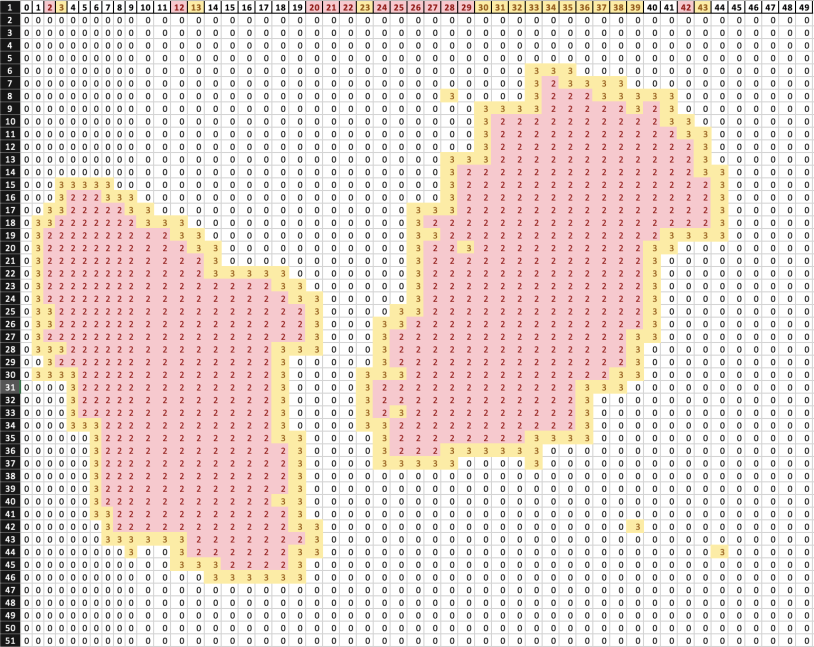
\includegraphics[scale=0.3]{DEFINITIVO.png}
    \caption{Edificios obtenidos}
\end{figure} 


\subsection{Análisis}
Luego de haber ejecutado el modelo en múltiples ocasiones, de vez en cuando (menos veces que la entrega pasada), el modelo no es capaz de ubicar correctamente ciertos nodos, pues de vez en cuando
los sitúa en lugares en los que no debería, es decir, que no se están cumpliendo ciertas restricciones. De las veces que iteramos, nos pudimos dar cuenta de que cuando la matriz es relativamente pequeña (menor a 30 x 30)
el modelo se resuelve \textbf{muy} rápido (menos de 1 segundo), sin embargo, a medida que se aumentan ciertos parámetros, como la dimensión de la matriz, demanda, o área mínima por habitante, el modelo simplemente
se demora \textbf{mucho} tiempo en entregar una solución, si es que entrega una, cuando demoraba mucho de lleno cortabamos la ejecución del modelo (cuando llevaba más de 15 minutos). Así, de forma empírica, 
notamos que el modelo es muy sensible a cambios en parámetros que son de revelancia. \newline \newline

Respecto a la solución obtenida, si bien podría ser intuitivo que mientras se necesite ubicar a una mayor cantidad de gente, puede que sea más difícil resolverlo el modelo, en este caso ocurrio lo contrario,
pues cuando disminuimos de la demanda igual a 500, a 350, el modelo simplemente demoraba mucho en procesar en cada iteración, así tuvimos que abortar su ejecución dado que no estaba entregando soluciones. A su vez,
es importante mencionar que entre iteración con distintos parámetros, el modelo puede variar drásticamente el tiempo de ejecución, desconocemos la razón de esto, pues de vez en cuando demora muy poco y al cambiar
un poquito ciertos parámetros, puede demorar mucho.


\section{Análisis de sensibilidad}
Al trabajar con el modelo y perturbar ciertos parámetros en específico, este da cuenta el grado de sensibilidad presentado ante el cambio de cada uno de ellos. Para el caso del cambio del lado derecho de la restricción 
correspondiente al cumpliemento de área mínima por habitante, en la restricción 8, este valor es sumamente influyente a los resultado del modelo. Incluso, un pequeño cambio en el valor del área mínima por habitante puede 
convertir el problema en infactible. También es relevante mencionar que el área mínima por habitante debe ser un valor real y lo suficientemente alto tal que no se generen edificaciones con superficies demasiado pequeñas 
en relación con la cantidad de personas que la habitan. Por ejemplo, un valor considerado como estándar y que es suficiente es de $11 m^2$ por habitante. En cuanto al cambio del parámetro correspondiente al presupuesto, 
en la restricción 9, se observó que al realizar ciertas modificaciones significativas en él, se producía un gran cambio a la hora de resolver el modelo. Si bien este no actuó de manera tan sensible ante la modificación 
como ante al cambio de área, de igual manera se vio perturbado el resultado, dejando a la vista significativas diferencias en los valores de las variables obtenidos. Es por esto que el valor otorgado al presupuesto
es importante, ya que al existir mayor cantidad monetaria, hay mayor probabilidad de que se pueda construir una edificación más grande, o con materiales más elevados en precio, pero que contaminen menos, generando
un cambio así en la decisión de que materiales utilizar por piso, y finalmente, en el valor óptimo obtenido en cuanto a la contaminación per cápita de $CO_2$. Finalmente, respecto al cambio en el parámetro $D$ que es la demanda 
habitacional, en la restricción 10, se pudo apreciar que al efectuar cambios menores en éste modelo pasaba a ser infactible, es por esto que se puede deducir que es altamente sensible. Es importante mencionar que la demanda 
habitacional es sumamente importante puesto que muchas veces se va a querer albergar a más personas en el proyecto habitacional y según lo mencionado anteriormente resulta ser muy complicado que se pueda realizar.\\




La alta sensibilidad presentada ante el cambio en el área mínima por habitante se ve explicada por el hecho de que tanto la demanda habitacional como el presupuesto se mantienen fijos, por lo tanto, se le estaría
exigiendo al modelo que entregue una solución que otorgue una mayor cantidad de área por persona, para la misma cantidad de personas y presupuesto. Justamente por lo anterior, es muy probable el hecho de aparición
de infactibilidad, ya que quizás a causa de que el presupuesto es el mismo, no existiría manera de aumentar la cantidad construida, y por tanto, no se podría cumplir con el área mínima solicitada. De igual manera,
a causa de que la demanda de personas sigue manteniéndose, no sería posible ubicar a toda esta población con la nueva área mínima exigida, si no que se quedarían algunos fuera sin poder ser ubicados, esto podría
ser la otra causa directa de la infactibilidad arrojada por el modelo. \newline \newline

En cuanto al análisis de las restricciones, se hace prácticamente imposible el estudio de todas ellas, ya que en su totalidad llegan a una cifra mayor a \textbf{36.000} (específicamente 36.512 para este set de datos)
y de estas, \textbf{12.734 están activas}, por lo que es imposible poner todas las restricciones activas y analizarlas de una manera breve en este documento. Si bien se intentó hacer un análisis de sensibilidad de la forma
más metódica y rigurosa posible con los comandos que provee Gurobi, esto no pudo ser posible debido a que nuestro modelo es del tipo MIP (Mixed-Integer Programming) y las formas que provee Gurobi para poder hacer
análisis de sensibilidad, funciona únicamente (de momento), para modelos continuos. Por lo que no se pudo realizar un análisis más detallista y estructurado, como al grupo le hubiese gustado. \newline \newline

Es relevante mencionar, que prácticamente la mayoría de las restricciones asociadas a personas o área, son sumamente sensibles frente a cambios leves en sus valores. Pudiendo influir al punto tal que el modelo
se vuelve infactible

\section{Conclusiones}
Realizar las actividades que siempre se han realizado pero de forma sustentable es uno de los mayores desafíos que la humanidad enfrenta actualmente. Este proyecto busca
aportar en la realización sustentable de la construcción, específicamente diseñando un proyecto inmobiliario lo más limpio posible bajo ciertas condiciones y recursos.
Los aspectos sobre los que se deciden al diseñar una construcción son varios y abordarlos todos es sumamente complejo desde el punto de vista de la programación lineal.\\

Nuestro modelo logra decidir sobre ciertas características de un proyecto inmobiliario pero que hay otras sobre las que solamense se supone o se consideran como datos
entregados al modelo (parámetros) para poder simplificarlo notablemente y mantener su linealidad. Es por esto que el modelo no es una representación muy precisa
de la realidad pues no permite decidir sobre muchos aspectos que podrían ser de interés, pero ello no implica que no sea útil. Más bien, el modelo sigue siendo útil
en cuanto a toma de decisiones, pues sí permite encontrar la mejor forma de disponer una cierta cantidad de edificaciones en un terreno determinado para suplir cierta
demanda habitacional, todo en base a requerimientos impuestos. Además, nuestro modelo puede ser una base simple para modelos más complejos (no lineales) que permitan
decidir sobre más aspectos (cantidad de pisos, cantidad de departamentos por piso, cantidad de edificaciones, entre otros). \newline \newline

A lo largo del desarrollo del modelo se presentaron diversos obstáculos que se tuvieron que resolver. Uno de ellos es la influencia del parámetro de área mínima por habitante
en el modelo. Considerando todos los parámetros constantes, excepto la cantidad de aŕea mínima por habitante, el modelo es muy sensible a los cambios marginales en este parámetro,
pues no se puede aumentar mucho ya que sino se vuelve infactible. Cada vez que se aumentaba un poco, la cantidad de área mínima por habitante que el modelo destinó para esos valores
de parámetros estaba muy cerca a la cantidad mínima.\\

Otro desafío fue la búsqueda de datos reales porque varios parámetros del modelo son difíciles de obtener y en la realidad dependen de muchos factores, como la emisión de $CO_2$ de 
ciertos materiales o la cantidad necesaria a utilizar de ciertos materiales. Un desafío presentado fue también la inclusión de aspectos estructurales en el modelo, lo que incluso en 
ciertos casos no fue posible.\\

Las principales lecciones obtenidas a lo largo del proyecto son varias. Una de las más importantes a nuestro parecer es intentar solucionar la no linealidad que aparecía de froma natural 
en el modelo, como el cálculo del área y en la multiplicación de variables relacionadas con la cantidad de material y pisos. La primera de ellas, el cálculo del área, fue bastante difícil 
de resolver en un principio, pero dada la estructura del modelo se pudo sortear gracias al emblemático Teorema de Pick, que permite calcular áreas de forma discreta con nodos interiores y 
exteriores, que es justamente la base del funcionamiento de nuestro modelo. Por medio del uso de este teorema, la problemática que surgió pudo ser solucionada. Respecto a la segunda problemática, 
lamentablemente no se pudo encontrar una forma de solucionarlo, por lo que forzosamente hubo que fijar como parámetro lo que en un principio estaba fijado como una variable (cantidad de pisos de un
edificio), para así no perder la linealidad, de lo contrario no hubiese sido posible mantener la linealidad exigida en el proyecto. Algo que es rescatable es que, como grupo al momento de analizar 
las restricciones una a una, vimos una que podría haber causado grandes problemas (pero que era necesaria), pues tenía que hacer una cantidad muy grande de combinaciones en cada iteración, para cada 
edificio, lo que en cuanto a tiempo	se refiere lo hacía inviable para ser resuelto en menos de 30 minutos.\\

Respecto a las soluciones obtenidas, es curioso que la mayor cantidad de veces, el modelo elegía construir la menor cantidad de edificios posible, pero con el área máxima permitida. A su vez, 
nos parece contraintuitivo y no podemos encontrar explicación, de que una vez construido el/los edificios(s), habían muchos nodos que no respetaban las condiciones de que tenían que estar rodeados 
por nodos interiores y exteriores, pues quedaban "sueltos" en el mapa/matriz. Luego de haber hecho exhaustivos análisis, no pudimos encontrar que podía estar causando tal situación, pues creemos que 
las restricciones, nuevamente, no pudimos encontrar una explicación. Sin embargo, nuestra hipótesis es que esto se puede deber a que eliminamos la restrcción que se encargaba de revisar subsecciones 
de la matriz, pero para esto tenía que hacer muchas combinaciones. Se puede interpretar como una especie de trade-off, entre mayor robustez del modelo o entregar una solución en un tiempo razonable, 
en este caso, optamos por obtener una solución en un tiempo razonable, a costa de que se puedan producir errores como estos. Otro aspecto a considerar respecto a las soluciones entregadas por el modelo,
es el correspondiente a qué pasaría si aumentase la contaminación de CO2 en pos de que los habitantes viviesen menos hacinados, en este caso se esperaría, por ejemplo, que el modelo decida 
si construir un edificio más grande, quizás de igual manera más caro y contaminante, en pos de aumentar el área mínima por habitante, para que así no siempre se arroje el mismo tipo de solución "menos contaminante" sino que también
considere la importancia de otros aspectos relevantes.\\

Algo a mejorar sobre el modelo es la cantidad de aspectos sobre los que decide. Por ejemplo, agregar más variables como la cantidad de pisos o la cantidad de edificaciones	sumarían utilidad y realismo 
al modelo pero ello supone desafíos. Un desafío es agregar estas variables manteniendo la linealidad, lo que es sumamente difícil y si es que es posbile. Otro desafío es agregar esas variables, convirtiendo 
el modelo a uno no lineal, y resolverlo. Esto último puede llegar a ser complejo ya que el modelo actual ya es difícil de resolver con cierto tamaño de parámetros, como por ejemplo un terreno muy grande, 
por lo que su versión no lineal con más variables de decisión puede llegar a ser inmensamente difícil de resolver. Otro desafío, es que si en un futuro nos enfrentamos frente a modelos con más variables y 
más restricciones, en síntesis, más complejos, se debe tener en consideración el contar con un/unos computadores con alta capacidad computacional para así resolver los problemas en un tiempo razonable, pues 
los computadores con los que contamos nosotros pueden ser limitados en cuanto a capacidad de procesamiento. \newline \newline

Como grupo hemos aprendido mucho en el transcurso del proyecto y creemos firmemente que esta experiencia nos va a ayudar para tener una mejor comprensión de todos los pasos que se deben realizar en un proyecto
de optimización, dificultades a superar, además de poder entender modelos más complejos.

\newpage
\section{Bibliografía}

\bibliographystyle{unsrt}
\bibliography{bibliography.bib}


\end{document}